\subsection{Intelligence Artificielle et NPC}

    \vspace{0.5cm}
    \subsubsection{Première soutenance}
    \vspace{0.5cm}

        Pour rendre notre jeu plus vivant et permettre aux joueurs de se mêler à la foule,
        il nous fallait créer des IA se déplaçant dans la ville.
        Pour cela, nous avons décider d'utiliser des NavMesh pour créer des zones où les 
        NPC peuvent se balader d'un point à un autre.
        Pour ne pas rendre leur comportement linéaire et trop prévisible, ce qui gâcherait inéluctablement le jeu,
        ils se déplacent de manière aléatoire  vers un point quelconque défini dans une liste de coordonnées.
        Les NPC ont donc des comportements pseudo-aléatoires (même s'ils empruntent toujours le chemin le plus court entre deux objectifs) qui permettent
        aux joueurs de se fondre plus facilement dans la masse. En d'autres termes, en faisait se comporter les IA comme des joueurs, on évite aux joueurs
        d'avoir à se comporter comme des robots.

        L’outil de navigation est assez poussé, et permet de définir les dimensions des personnages,
        ainsi que la hauteur de laquelle ils peuvent sauter et les pentes qu’ils peuvent emprunter.
        Ici, la pente maximale est de 33.4°, mais si ce chiffre avait été plus élevé,
        les pentes seraient devenues praticables (bleues)\footnote{Voir fugure 3}, et les personnages auraient pu
        monter sans utiliser les escaliers (ce qui n’est évidemment pas le but).


        Pour rendre ces IA plus humaines, les joueurs peuvent les bousculer et les étourdir en courant vers eux.
        Ils reprenent leur trajet au bout de quelques secondes. Il faudra ainsi, dans les prochaines versions, 
        améliorer la navigation afin que le chemin emprunté ne soit pas toujours le plus court. 
        

        \begin{figure}[!hbt]
                \centering
                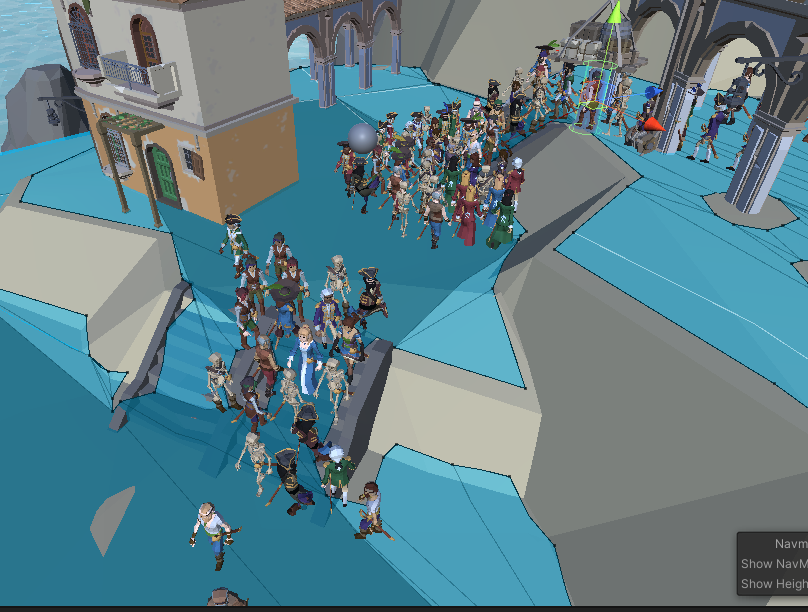
\includegraphics[scale=0.3]{ia_stairs_bug.png}
                \caption{Problème rencontré lorsque de nombreuses IA vont au même endroit}
        \end{figure}
        \FloatBarrier

    \vspace{0.5cm}
    \subsubsection{Deuxième soutenance}
    \vspace{0.5cm}


        Nous avons essayé plusieurs types de déplacement pour les IA. Nous avons fait des NPC zones qui permettent de créer des quartiers
        où les NPC peuvent se balader librement dans la zone. Si un NPC est tué dans la zone, un nouveau apparait avec un effet visuel 
        approprié (shader d'apparition).
        

        Pour le système de déplacement de l'IA,
        nous avons essayé plusieurs algorithmes différents :
        
        \begin{itemize}
            \item Le premier algorithme que nous avions montré lors de la première soutenance
            était un déplacement vers un élément alétoire d'une liste de coordonnées prédéfinie.
            Le tracé était de ce fait trop prévisible et ne permettait pas de se déplacer librement en restant discret.
            De plus, si un personnage allait d'un point A vers un point B, et un autre de B vers A,
            alors prenant le chemin le plus court ils finissaient par se croiser (face à face) et finir coincés.
            
            \item Nous avons donc décidé de rajouter plus d'aléatoire dans leurs déplacements. Les IA cherchent 
            une destination "accessible" dans un rayon proche. Le problème était que la librairie Unity AI intégrée 
            cherche un chemin complet ou partiel. Le rendu final montrait des personnages qui finissaient toujours 
            par être attirés par les bordures de la carte.

            \item Le dernier système intégré cherche une destination dans une certaine zone.
            Au lieu de chercher un point proche de lui, il cherche un chemin vers une destination aléatoire, 
            et recommence lorsque ce point est atteint ou si aucun chemin complet n'a été trouvé.
        \end{itemize}
            

        \begin{figure}[hbt!]
            \centering
            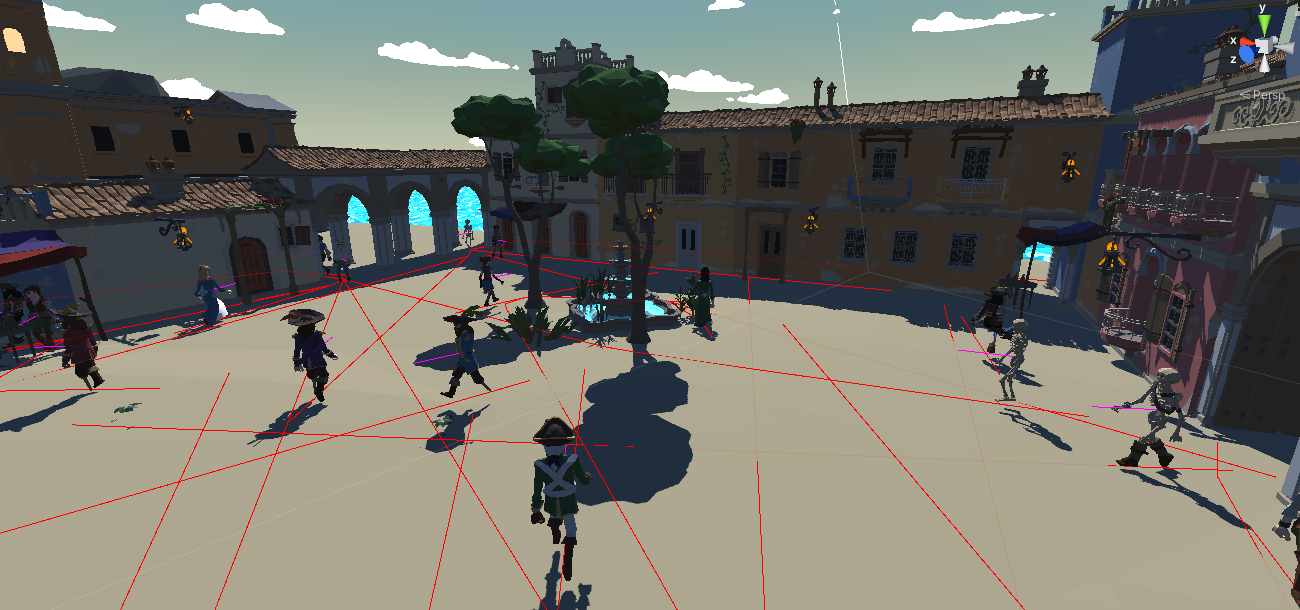
\includegraphics[scale=0.43]{navmesh_path.png}
            \caption{Représentation vectorielle des path des IA}
        \end{figure}
        \FloatBarrier
        
    
        Afin de rendre les IA moins scriptées, nous avons ajouté des événements aléatoires.
        
        En outre, des zones de discussion ont été implémentées : ce sont des zones où les joueurs et le NPC peuvent interagir 
        et se fondre dans la discussion pour se cacher. Les IA qui les traversent s'y arrêtent, parlent,avant de repartir au bout d'une durée 
        de temps aléatoire.

        \begin{figure}[hbt!]
            \centering
            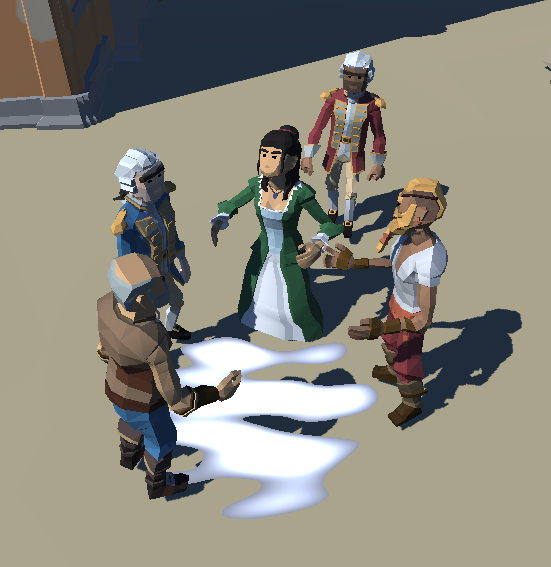
\includegraphics[scale=0.5]{talk_zone.png}
            \caption{Zone de discussion}
        \end{figure}
        \FloatBarrier


    \vspace{0.5cm}
    \subsubsection{Dernière soutenance}
    \vspace{0.5cm}

        \paragraph{Optimisation de l'algorithme de déplacement}

        Avec l'algorithme de navigation des NPC précédent, ces derniers recherchaient un nouveau point après avoir atteint 
        le leur, ce qui posait des problèmes car les IA s'arrêtaient quelques instants pour calculer leur destination. Cette dernière 
        est maintenant calculée lorsqu'un avancement de deux tiers est atteint sur le trajet. Cela permet d'éviter ces moments 
        d'inactivité. Le mode de recherche a aussi connu de très légères optimisations.